\documentclass[12pt,twoside,english]{article}
\usepackage[utf8]{inputenc}
\usepackage[font=small,labelfont=bf]{caption}
%%%%%%%%%%%%%%%%%%%%%%%%%%%%%%%%%%%%%%%%%%%%%%%%%%%%%%%%%%%%%%%%%%%%%%%
%% template for II2202 proposal
%% original 2020.08.28
%% revised  
%%%%%%%%%%%%%%%%%%%%%%%%%%%%%%%%%%%%%%%%%%%%%%%%%%%%%%%%%%%%%%%%%%%%%%%
%

%%% Local Variables:
%%% mode: latex
%%% TeX-master: "."
%%% End:

%%TC:ignore
\usepackage[paper=a4paper,dvips,top=1.5cm,left=1.5cm,right=1.5cm,
    foot=1cm,bottom=1.5cm]{geometry}


\usepackage{todonotes}          %to provide inline and margin notes
%\usepackage[T1]{fontenc}
%%\usepackage{pslatex}
\renewcommand{\rmdefault}{ptm} 
\usepackage{mathptmx}
\usepackage[scaled=.90]{helvet}
\usepackage{courier}
%
\usepackage{bookmark}

\usepackage{fancyhdr}
\pagestyle{fancy}

%%----------------------------------------------------------------------------
%%   pcap2tex stuff
%%----------------------------------------------------------------------------
 %%\usepackage[dvipsnames*,svgnames]{xcolor} %% For extended colors
 %%\usepackage{tikz}  %% Already loaded
 %%\usetikzlibrary{arrows,decorations.pathmorphing,backgrounds,fit,positioning,calc,shapes}

%% \usepackage{pgfmath}	% --math engine
%%----------------------------------------------------------------------------
%% \usepackage[latin1]{inputenc}
\usepackage[utf8]{inputenc} % inputenc allows the user to input accented characters directly from the keyboard
\usepackage[english]{babel}
%% \usepackage{rotating}		 %% For text rotating
\usepackage{array}			 %% For table wrapping
\usepackage{graphicx}	                 %% Support for images
\usepackage{float}			 %% Suppor for more flexible floating box positioning
\usepackage{color}                       %% Support for colour 
\usepackage{mdwlist}
%% \usepackage{setspace}                 %% For fine-grained control over line spacing
%% \usepackage{listings}		 %% For source code listing
%% \usepackage{bytefield}                %% For packet drawings
\usepackage{tabularx}		         %% For simple table stretching
%%\usepackage{multirow}	                 %% Support for multirow colums in tables
\usepackage{dcolumn}	                 %% Support for decimal point alignment in tables
\usepackage{url}	                 %% Support for breaking URLs
\usepackage[perpage,para,symbol]{footmisc} %% use symbols to ``number'' footnotes and reset which symbol is used first on each page
\usepackage[binary-units=true]{siunitx} %% to be able to use binary units
\newcommand{\SIadj}[2]{\SI[number-unit-product={\text{-}}]{#1}{#2}}

%% \usepackage{pygmentize}           %% required to use minted -- see python-pygments - Pygments is a Syntax Highlighting Package written in Python
%% \usepackage{minted}		     %% For source code highlighting

%% \usepackage{hyperref}		
\usepackage[all]{hypcap}	 %% Prevents an issue related to hyperref and caption linking
%% setup hyperref to use the darkblue color on links
%% \hypersetup{colorlinks,breaklinks,
%%             linkcolor=darkblue,urlcolor=darkblue,
%%             anchorcolor=darkblue,citecolor=darkblue}

%% Some definitions of used colors
\definecolor{darkblue}{rgb}{0.0,0.0,0.3} %% define a color called darkblue
\definecolor{darkred}{rgb}{0.4,0.0,0.0}
\definecolor{red}{rgb}{0.7,0.0,0.0}
\definecolor{lightgrey}{rgb}{0.8,0.8,0.8} 
\definecolor{grey}{rgb}{0.6,0.6,0.6}
\definecolor{darkgrey}{rgb}{0.4,0.4,0.4}
%% Reduce hyphenation as much as possible
\hyphenpenalty=15000 
\tolerance=1000

%% useful redefinitions to use with tables
\newcommand{\rr}{\raggedright} %% raggedright command redefinition
\newcommand{\rl}{\raggedleft} %% raggedleft command redefinition
\newcommand{\tn}{\tabularnewline} %% tabularnewline command redefinition

%% definition of new command for bytefield package
\newcommand{\colorbitbox}[3]{%
	\rlap{\bitbox{#2}{\color{#1}\rule{\width}{\height}}}%
	\bitbox{#2}{#3}}

%% command to ease switching to red color text
\newcommand{\red}{\color{red}}
%%redefinition of paragraph command to insert a breakline after it
\makeatletter
\renewcommand\paragraph{\@startsection{paragraph}{4}{\z@}%
  {-3.25ex\@plus -1ex \@minus -.2ex}%
  {1.5ex \@plus .2ex}%
  {\normalfont\normalsize\bfseries}}
\makeatother

%%redefinition of subparagraph command to insert a breakline after it
\makeatletter
\renewcommand\subparagraph{\@startsection{subparagraph}{5}{\z@}%
  {-3.25ex\@plus -1ex \@minus -.2ex}%
  {1.5ex \@plus .2ex}%
  {\normalfont\normalsize\bfseries}}
\makeatother

\setcounter{tocdepth}{3}	%% 3 depth levels in TOC
\setcounter{secnumdepth}{5}
%% Acronyms
\usepackage[acronym, nopostdot]{glossaries}
\glsdisablehyper
\makeglossaries

\renewcommand{\headrulewidth}{0pt}
%%%%%%%%%%%%%%%%%%%%%%%%%%%%%%%%%%%%%%%%%%%%%%%%%%%%%%%%%%%%%%%%%%%%
%% End of preamble
%%%%%%%%%%%%%%%%%%%%%%%%%%%%%%%%%%%%%%%%%%%%%%%%%%%%%%%%%%%%%%%%%%%%

\newacronym{AR}{AR}{augmented reality}

% Keywords command
\providecommand{\keywords}[1]
{
  \small	
  \textbf{\textit{Keywords:}} #1
}

\title{Trade-offs Between Immersion and Energy Consumption With Automatic Naturalistic Lighting in Augmented Reality: A Pre-Study}
\author{
        \textsc{Stefano Formicola}
            \qquad
        \textsc{Christoph Albert Johns}
        \mbox{}\\
        \normalsize
            \texttt{formico}
        \textbar{}
            \texttt{cajohns}
        \normalsize
            \texttt{@kth.se}
}
\date{\today}


\lhead{II2202, Fall 2020, Period 1-2}
%% or \lhead{II2202, Fall 2020, Period 1}
\chead{Project Report}
\rhead{\date{\today}}

\makeatletter
\let\ps@plain\ps@fancy 
\makeatother

\setlength{\headheight}{15pt}
\begin{document}

\maketitle


\begin{abstract}
\label{sec:abstract}

This research project investigates the effect of automatic naturalistic lighting in \gls{AR} applications on immersion and on energy consumption in a pre-study with seven participants.
A simple open-source card-matching game is modified to implement and control the corresponding rendering setting as provided by Apple's \gls{AR} \gls{API} RealityKit and tested with a small convenience sample of users.
A within-subject research design is chosen to measure immersion through the \gls{IEQ} while overall \gls{CPU} usage is monitored and logged for both test conditions in randomized order.
A Mann-Whitney-U-test is used to test for significant differences in immersion and \gls{CPU} usage between both conditions.
The preliminary results seem to suggest that immersion is not significantly affected by automatic naturalistic lighting whereas \gls{CPU} usage might be higher for the enabled condition, although a larger scale study is required for a more meaningful account.
For such a large-scale study, usability issues of the sample application should be resolved.
Additionally, it should be considered whether the \gls{IEQ} should be replaced with a questionnaire that is more specific to \gls{AR} applications.

\end{abstract}

%TC:ignore
\keywords{Augmented reality, Lighting, Immersion, Energy consumption}
%TC:endignore
\clearpage

\selectlanguage{english}
\tableofcontents

\section*{List of Acronyms and Abbreviations}
\label{list-of-acronyms-and-abbreviations}
\renewcommand{\glossarysection}[2][]{} %% skip the title
\printglossary[type=\acronymtype, nonumberlist]

\clearpage
\section{Introduction}
\label{sect:introduction}

% What is the problem?
Through the dissemination of powerful and easy-to-use framework \glsplural{API}, increasingly advanced features for \gls{AR} have become readily available to developers and designers.
Apple's \gls{AR} \gls{API} \textit{RealityKit}, for example, has enabled creators to easily add occlusion, video textures, and shared states for collaborative experiences to their \gls{AR} applications~\cite{apple_realitykit_2020-1}.
One of the especially notable new features of recent years has been real-time light estimation~\cite{apple_arlightestimate_2020}.
Applications that enable this feature --- or, as in the case of RealityKit, choose to keep this default setting --- gain access to information about a scene's lighting with every video frame that is delivered to the current session and can use this to apply dynamic shading to virtual objects matching the real-world lighting conditions~\cite{apple_arlightestimate_2020}.
To achieve this, camera-sensor data for one or multiple probes in the scene is continuously processed and evaluated~\cite{apple_arlightestimate_2020,apple_disablearenvironmentlighting_2020}.
This, depending on the scene and lighting conditions, can be a computationally intensive operation~\cite{steed_constructing_2016}.
Enabling automatic naturalistic lighting could, therefore, lead to increased scene realism at the cost of decreased energy efficiency.

This research aims at illuminating the relationship between immersion and energy consumption in deploying automatic naturalistic lighting, thus empowering developers and designers to decide the most appropriate feature sets for their applications considering both user experience and sustainability aspects.
For this, our project builds on two main lines of research: prior works evaluating the relationship between visual characteristics of \gls{AR} objects and user experience (e.g.~\cite{gabbard_effects_2006}) and research on the approximation of natural lighting conditions within virtual scenes in augmented reality (e.g.~\cite{aittala_inverse_2010}).
While there has been extensive research on the effect of design decisions on several aspects of user experience in digital games~\cite{johnson_validation_2018} --- even in \gls{AR} games (e.g.~\cite{georgiou_development_2017}) --- the effect of lighting and more specifically automatic naturalistic lighting in \gls{AR} games on immersion seems not to have been examined yet.

We chose to investigate the effect of automatic naturalistic lighting on immersion --- in contrast to, for example, \textit{flow}~\cite{csikszentmihalyi_flow_1990} --- because it is independent from optimal experience, which our method wasn't able to produce, and because it is very likely to relate to visual presentation and, therefore, lighting~\cite{jennett_measuring_2008}.
There exist multiple alternative measures that could have been chosen to explore aspects of the experience when playing video games instead (see~\cite{dey_systematic_2018, dunser_survey_2008} for overviews).
We reason, however, that immersion is an appropriate measure for this study since automatic naturalistic lighting is likely to enhance the sense of realism of a scene.
As Witmer and Singer argue, this sense of "scene realism" is one of the governing factors for presence in virtual environments~\cite{witmer_measuring_1998}, which in turn affects how immersive a virtual environment appears~\cite{jennett_measuring_2008}.

Since we were limited by our resources in terms of time and budget, however, and since this research project was conducted during the COVID-19 pandemic, we were not able to reach the necessary number of participants that would be required to fully illuminate said relationship.
Instead, we focused on conducting a smaller scale pre-study that can give some indication about the results as well as provide some insights into the suitability of our chosen methods and tools.
The deliverables of our project are, therefore: an example \gls{AR} application to measure immersion levels and monitor energy consumption, a tested and evaluated method (setup, procedure, and analysis) for a full-scale study and an indication for the results of said study.

\subsection{Research Questions}

% What are the research questions?
For this pre-study as well as for the eventual full-scale study, we are interested in two major research questions relating to one of the two aspects of our investigation each: automatic naturalistic lighting's effect on immersion and its effect on energy consumption.
More specifically, we want to examine users' perceived immersion when they are explicitly asked to rate said experience using a standardized questionnaire (i.e. the \gls{IEQ} developed by Jennett et al.~\cite{jennett_measuring_2008}) as well as their own unsupported articulation of any difference between enabled and disabled automatic naturalistic lighting.
Additionally, we want to explore the effect of automatic naturalistic lighting on device metrics collected in the background that can give an indication about the condition's effect on device resource utilization.
Overall, we proposed to investigate the following questions:

\begin{description}
    \item[RQ1.] Do users experience a difference in immersion between enabled and disabled automatic naturalistic lighting?
    \item[RQ1a.] If they perceive a difference, are the participants able to tell that lighting is the cause?
    \item[RQ2.] How does enabling automatic naturalistic lighting affect \gls{CPU} usage?
\end{description}

In our pre-study, energy consumption has been measured in terms of \gls{CPU} usage because it can very finely be measured on the test device in contrast to general energy consumption.

\subsection{Research Hypotheses}

While we are aware that we were only able to test the proposed method on a small scale, we hypothesize the following outcomes for a full-scale experiment:

\begin{description}
    \item[H1.] Users experience higher immersion levels when automatic naturalistic lighting is enabled.
    \item[H1a.] Users are able to tell that the lighting was different between both runs of the experiment.
    \item[H2.] \gls{CPU} usage is higher when automatic naturalistic lighting is enabled.
\end{description}

As has been explained above, scene realism is positively correlated with presence and thereby immersion.
That is why we expect the lighting condition that more closely matches the scene's natural environment to lead to higher levels of immersion, resulting in the first hypothesis.
Second, because the difference between both conditions lies in a salient visual feature which affects \gls{AR} objects' color and reflections, we expect not only the indirect measure of immersion as assessed through the \gls{IEQ} to be affected.
We instead hypothesize that users will recognize the difference between both conditions and will be able to articulate how they differ without support from the examiner.
And finally, regarding the energy impact of automatic naturalistic lighting, we expect the computationally intensive continuous probing and estimation of the \gls{AR} scenes environment lighting to lead to higher levels of overall \gls{CPU} usage.


\section{Method}
\label{sect:method}

We propose a within-subject design to test the effects of the two conditions \textit{automatic naturalistic lighting enabled} and \textit{automatic naturalistic lighting disabled} on immersion using the \gls{IEQ} developed by Jennett et al.~\cite{jennett_measuring_2008} while measuring \gls{CPU} usage via a device metrics logging tool in combination with a sample \gls{AR} application.
For this, we modified an existing open source mobile \gls{AR} game and prepared a form that includes the \gls{IEQ}, while Xcode's Developer Tools' \textit{Instruments} were used to measure \gls{CPU} usage over time.
Because of its popularity across countries and languages, we considered the game \textit{Memory} or \textit{Concentration}, in which players have to remember the order and color of different cards, a valid candidate for the experiment.
The implementation was done for iOS devices and developed on Apple's \gls{IDE} Xcode using the ARKit and RealityKit \glsplural{API}.
The experiment consisted of one three-minute session of gameplay for each condition, with and without the automatic naturalistic lighting, per subject.
The user interface included a toggle button hidden from the player to enable and disable the automatic naturalistic lighting feature for the two runs of the experiment (see Figure \ref{fig:sample_app_comparison} for a comparison between enabled and disabled automatic naturalistic lighting in the sample application).
In the following, the participant profile, procedure, data collection, and analysis are described.

\begin{figure}[h]
    \centering
    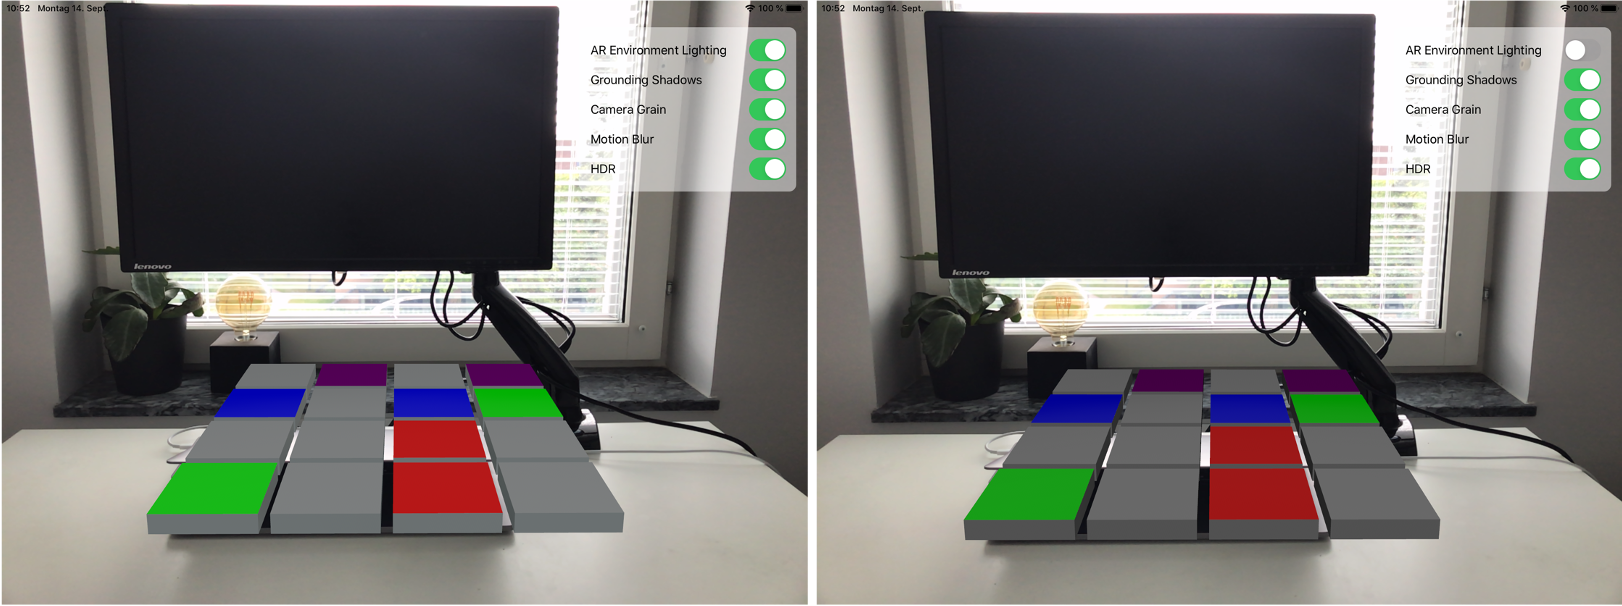
\includegraphics[width=0.7\textwidth]{imgs/sample_app_comparison.png}
    \caption{Comparison between enabled (left) and disabled (right) automatic naturalistic lighting in the sample card-matching \gls{AR} application. The controls can be hidden before the test device is handed over to the participant.}
    \label{fig:sample_app_comparison}
\end{figure}

\subsection{Participants}
\label{sect:participants}

The participants were recruited via an opportunity sample and were---due to the difficulties and restrictions regarding gatherings of people during the COVID-19 pandemic---mostly international students living on campus at a major technical university in Sweden.
To limit the effect of novelty on immersion levels, they were required to have had played a card-matching game similar to the sample game before.
It was, however, not required for participants to have played a digital version of this game before taking part in the experiment.
To further mitigate the effect of novelty, participants were required to have experienced an \gls{AR} scene on a mobile handheld device before.
Overall, seven participants took part in this study.
They had an average age of 24.7 (SD = 1.60), ranging from 23 to 28 years.
All seven participants were male.

\subsection{Preparations}
\label{sect:preparations}

To be able to conduct the proposed experiment, we prepared an example application that could easily control the currently active lighting setting and a digital questionnaire that included a consent form as well as the \gls{IEQ}.

We modified an open-source \gls{AR} card-matching game~\cite{cobb_maxxfrazerrealitykit-cardflip_2020} to include an option to enable and disable automatic naturalistic lighting using RealityKit's \textit{.disableAREnvironmentLighting} render option.
The application was then installed on an Apple iPad Pro 2017 (model number FPDY2FD/A) so it could be presented to participants and monitored using the Xcode \gls{IDE}.
The application that formed the basis for our experiment was chosen due to its simplicity in functionality and visual presentation as well as participants' general familiarity with the underlying game of \textit{Concentration}, thereby reducing the risk of errors in use or unwanted effects on immersion due to scene complexity or novelty.
Additionally, several suitable rooms accessible to students were identified so the experiment could be conducted in an indoor setting with controlled lighting.

To collect consent as well as immersion data using the \gls{IEQ}, a Google Forms document was prepared that informed participants about the purpose of the experiment as well as the kind of data that would be collected, stored, and analyzed (see Appendix~\ref{sect:consent-form}).
Additionally, it included two instances of the \gls{IEQ} developed by Jennett et al.~\cite{jennett_measuring_2008} to collect data on players' immersion levels for each of the two lighting conditions.
The full extent of the \gls{IEQ} as used in this experiment can be found in Appendix~\ref{sect:ieq}.

\subsection{Procedure}
\label{sect:procedure}

Before the start of the experiment, participants were informed about the collection of data regarding the device activity and their questionnaire answers after both runs of the game.
Moreover, their right to withdraw from the experiment at any time was clarified as well as the possibility to ask for the deletion of all data associated with their person.
The purpose of the experiment was stated to the participants in general terms as "investigating immersion in \gls{AR} games" to avoid influencing their perception of the scene by directing their attention towards lighting. 
They were asked to fill the consent form detailed above.

To further mitigate the risk of influencing participants and to address the concerns brought up by Jennett et al.~\cite{jennett_measuring_2008} regarding the effect of prior experience on immersion, participants were then given a trial period with a third lighting condition: disabled automatic naturalistic lighting and an added point light above the scene.
After they had indicated to sufficiently understand the experiment application, participants were asked to complete as many rounds of the card-matching game with as few errors as possible, before they were interrupted after three minutes and the render option was changed for the second run following the study design of Jennett et al.~\cite{jennett_measuring_2008}.
The motivation for this experiment design was to allow for a more challenging experience across player ability levels, thereby increasing flow~\cite{csikszentmihalyi_flow_1990} and general immersion levels as well as reducing overall variance in immersion~\cite{jennett_measuring_2008}.
The order of both render options was randomized to improve reliability and participants were not informed about the currently active render option to avoid biases.
The first run was considered started after the participants indicated that they were ready for the experiment to begin.

During each run of the experiment, the \gls{IDE} Xcode and more specifically its \textit{Instruments} feature~\cite{apple_xcode_2020} were used to log the test device's \gls{CPU} utilization in three second intervals according to Apple's type definitions~\cite{apple_system_2020}.
While there exists a more general power metric that can be logged through the same application~\cite{apple_energy_2020-1}, that metric is discrete, abstract, and too inaccurate to be elastic towards enabled and disabled automatic naturalistic lighting and was, therefore, not used.
We decided not to have participants think aloud during their app usage to avoid unwanted effects on their immersion~\cite{van_den_haak_retrospective_2003}.

After each run, participants were asked to fill out the \gls{IEQ} detailed above to measure their levels of immersion dependent on the lighting treatment.
After the second run, participants were additionally asked about their general experience using the application and to elaborate on any differences they noticed between both runs.
While alternatives such as tracking eye movement or measuring reaction times could also have been used to measure immersion~\cite{jennett_measuring_2008}, we chose a questionnaire approach as the most economical option that still has satisfactory precedence in literature~\cite{boyle_engagement_2012}.
If a participant referred to "light", "lighting", "color", or "contrast" while answering the open questions in the questionnaire, the difference in lighting was considered as noticed by the user.

After the experiment was completed, participants were debriefed and fully informed about the purpose of the study and given the opportunity to withdraw their consent.
The duration of the experiment per participant was around twenty minutes.

\subsection{Data analysis}
\label{sect:data_analysis}

After the above data had been successfully gathered, we conducted a statistical analysis regarding the participants' immersion levels and the \gls{CPU} usage between both lighting conditions using a Mann-Whitney U-test to check for significant differences.
We chose this test because it does not require a normal distribution and because it was used by Jennett et al. in their original studies on immersion~\cite{jennett_measuring_2008}.
However, the Student's \textit{t}-test's could also have been used---as for example Nordin et al.~\cite{nordin_attention_2013} did in their immersion experiments---, if the data were normally distributed.
All statistical analysis was performed using Python 3.8.3 with the packages Pandas 1.1.4 and SciPy 1.5.4.
All visualizations were created using Seaborn 0.11.0.
Additionally, we report the results of the open questions.

We are aware that neither the results of our statistical analysis nor those of our qualitative research should be used to infer knowledge about either the effect of automatic naturalistic lighting on immersion or energy consumption due to the small sample size.
Rather, the analysis can give some indication as to the results of a full-scale study as well as enable us to evaluate the chosen methods and tools.

\section{Results}
\label{sect:results}

The immersion scores per question according to the \gls{IEQ} were calculated as ranging from a 1 for strongly disagree to a 5 for strongly agree.
Scores for positively formulated questions were added, while scores for negatively formulated questions were subtracted to calculate the overall immersion score per participant and condition.
Overall \gls{CPU} usage at a given time was calculated by adding the \gls{CPU} usage percentages for all activity kinds with the same timestamp.
Since the System CPU Percentage Engineering Type~\cite{apple_system_2020} has a range from 0\% to 100\% multiplied by the number of \gls{CPU} cores in the given device, this can result in values exceeding 100\% (or 1 as in the formatting of our analysis).

Contrary to our first hypothesis \textbf{H1}, overall immersion scores did not differ significantly between both conditions (Mann-Whitney $ U = 18.5 $, $ p = 0.241 $) with the mean overall immersion score for the automatic naturalistic lighting \textit{disabled} condition of 76.0 (SD = 6.6) even slightly exceeding the \textit{enabled} condition with 74.7 (SD = 7.3) (see Figure \ref{fig:immersion_plot}).

\begin{figure}[h]
    \centering
    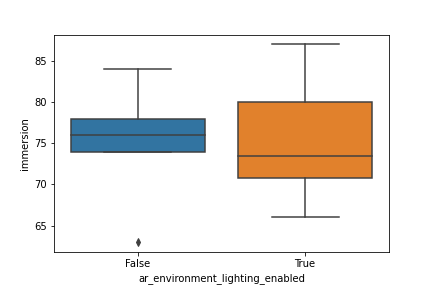
\includegraphics[width=0.5\textwidth]{imgs/immersion_plot}
    \caption{Immersion scores for the disabled and enabled conditions in our small pre-study ($ N = 7 $).}
    \label{fig:immersion_plot}
\end{figure}

Regarding hypothesis \textbf{H1a}, there was no indication whether most participants in a full-scale study would notice a difference between both conditions as three of the seven participants in our pre-study stated they had not noticed any distinction.
Within the group of participants that had answered to have noticed a difference, the immersion scores between automatic naturalistic lighting enabled and disabled did not differ significantly (Mann-Whitney $ U = 4.0 $, $ p = 0.155 $) with mean immersion scores of 76.3 (SD = 4.9) for the enabled and 76.0 (SD = 11.4) for the disabled condition respectively.

Finally, contrary to our hypothesis \textbf{H2}, mean \gls{CPU} usage did not significantly differ between both conditions (Mann-Whitney $ U = 16.0 $, $ p = 0.405 $) with 61.8\% (SD = 6.7\%) mean overall \gls{CPU} usage in the disabled condition and 63.1\% (SD = 6.6\%) in the enabled condition.
However, as can be seen in Figure \ref{fig:cpu_raw_plot}, the distributions of overall \gls{CPU} usage per condition across all experiments (i.e. without calculating a mean per experiment and condition first) did appear different.
The enabled condition resulted in a significantly higher overall \gls{CPU} usage even in our small pre-study (Mann-Whitney $ U = 53272.5 $, $ p = 0.029 $).

\begin{figure}[h]
    \centering
    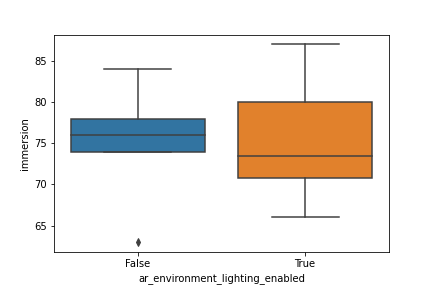
\includegraphics[width=0.5\textwidth]{imgs/cpu_raw_plot}
    \caption{Overall \gls{CPU} usage for the disabled and enabled conditions. The overall \gls{CPU} usage can exceed 1 for devices with more than one \gls{CPU} core (range from 0 to number of cores) as specified in the corresponding data type definition of the logging software~\cite{apple_system_2020}.}
    \label{fig:cpu_raw_plot}
\end{figure}


\section{Discussion}
\label{sect:discussion}

The results of our pre-study seem to indicate that there might not be a trade-off between improving immersion and increasing energy consumption when deploying automatic naturalistic lighting.
Instead, it appears that immersion is largely unaffected by the feature while energy consumption as measured through \gls{CPU} usage in our experiment might be slightly increased.
This would lead us to conclude that automatic naturalistic lighting should not be employed by designers and developers, so that users' battery can be preserved or computational resources can be freed for alternative uses.
We need, however, to look at the results in more detail to justify this conclusion.

As our results regarding hypothesis \textbf{H1} show, the immersion scores for our seven participants did not significantly differ between enabled and disabled automatic naturalistic lighting.
We instead observed a quite wide distribution for both conditions ($ SD_{enabled} = 7.3 $, $ SD_{disabled} = 6.7 $).
This could indicate that the difference between both lighting conditions is hardly perceivable when not put side by side and that other factors such as changes in the environment (e.g. noises or a change in natural lighting) diminish automatic naturalistic lighting's effect on immersion.
This is further supported by our results regarding hypothesis \textbf{H1a}.

According to the questionnaire data as well as the comments from our study participants, the visual characteristics of the scene did not appear noticeably different between both conditions.
Even when the setup of the experiment was explained to the participants, some could not recall any difference in appearance between the conditions.
Only when toggling the corresponding render setting for a live scene resulting in an immediate change, the participants were able to recognize that the virtual objects were lit differently.
Similarly, the immersion scores for both groups–-those participants who claimed to have noticed a difference between both conditions and those who had not---did not differ significantly.
It seems that the hypothesized improvement in scene realism brought about by automatic naturalistic lighting was not strong enough in our chosen application to be consciously perceived or to result in increased immersion as measured through the \gls{IEQ}.

A similar impression emerges when examining \gls{CPU} usage:
Taking only the overall mean utilization into consideration, we would have to reject our hypothesis \textbf{H2}.
Mean \gls{CPU} usage appears largely unaffected by enabling or disabling automatic naturalistic lighting with the results of our Mann-Whitney U-test showing no significant difference between both conditions and even the range of the two measurements being remarkably similar (disabled: 53.2\% to 70.1\%; enabled: 51.7\% to 71.3\%).
When considering the distribution of all \gls{CPU} usage data between both conditions, however (i.e. treating the overall \gls{CPU} usage at any point of time during all experiments the same without aggregating the data for an experiment first), a slight but significant increase during enabled automatic naturalistic lighting can be observed.
While this would generally support our hypothesis, the difference in \gls{CPU} usage is so small that it would likely not result in a perceivable difference in energy consumption or battery life for users of the sample application.
This conclusion would, however, need to be validated by another study.

This leaves us with the overall result of our pre-study:
While the difference between both conditions can be noticed in a side-by-side comparison, enabling or disabling automatic naturalistic lighting does not have a significant effect on the appearance of \gls{AR} scenes and consequently on immersion.
And, while it statistically could be argued---even with our small sample size---that \gls{CPU} usage and thereby energy consumption is affected by this choice, it would likely not result in a meaningful difference for the user experience of an \gls{AR} application.
It is, therefore, within designers' and developers' volition whether to enable or disable automatic naturalistic lighting for their applications according to their preferences or other decision factors than those examined in this study.

We are, however, aware of the numerous limitations of our pre-study and want to give as complete an account as possible of these weaknesses to prepare for a possible full-scale study with a greater number of participants investigating the same relationships.

\section{Limitations}
\label{sect:limitations}

The most pressing and most obvious limitation of our pre-study is the small sample size.
We were largely limited to descriptive statistics and tests with low statistical power due to the fact that we could only gather data from seven participants.
To reach higher levels of confidence, especially regarding any possible differences in immersion between both tested conditions, more participants would need to be recruited.
This would likely also address another major issue regarding our sample: the lack of diversity.
Due to our reliance on convenience sampling during a time where contact outside of one's immediate group of acquaintances is rather difficult or even prohibited, we were unable to recruit any female participants or participants outside the age range of students.
For a full-scale study, more emphasis should be put on gathering a sample representing a larger part of the potential user group of \gls{AR} applications.

The results might additionally be affected by the study design.
Some participants noted that asking about the overall experience and any differences between both runs of the experiment would lead to biased answers since it provoked answers even if the participant would not have experienced significant differences.
One participant suggested a third experiment variation in addition to the two randomized conditions tested in this study where the active render setting is not changed between both runs.
In addition to these weaknesses of our chosen method, we observed some weaknesses of our tooling as well.

While conducting the pre-study, we experienced some difficulties with our chosen software.
The modified sample application as well as the monitoring and logging software chosen had reliability issues that hindered the data gathering process.
In one of the experiments, logging of the \gls{CPU} usage suddenly stopped after circa 1.5~min.
While other data such as network events that were logged automatically by the software could still be accessed, \gls{CPU} data was non-retrievable.
In another experiment, the logging software suddenly exited after the tester requested to stop and save the recording.
Here again, \gls{CPU} data was non-retrievable.
The sample application, similarly, experienced some issues that seemed to relate to the Xcode \gls{IDE}.
In one experiment, the application failed to exit through the software and had to be manually shut down.
Regarding less severe concerns, the sample application appeared to lack in terms of its feedback mechanisms.
During multiple experiments, the probing phase (i.e. the phase during which the application gathers information about the environment, specifically to find a horizontal plane to use as an anchor for the virtual objects of the scene) which was indicated by an overlay with instructions to slowly move the device was exited without placing the virtual objects in an appropriate time frame.
No obvious cause or pattern to this behavior could be identified.
This lead to multiple restarts of the application which delayed several runs of the experiment.

During the experiments, several participants further experienced difficulties when interacting with the sample application.
Since the application does support scaling and positioning of the virtual objects during the setup phase for increased usability but does not save these settings, the virtual cards were displayed in the original scale and position after each successful game resulting in visible irritation by the participants.
Additionally, the participants seemed to experience some discomfort holding the test device as multiple participants frequently adjusted their grip during the second run of the experiment.
One participant even rested the device on a table to avoid having to hold it.
It was, furthermore, noticeable that all participants moved the device during the trial phase of the experiment and some at the beginning of the first run, but all stopped moving the device eventually.
They instead remained in a fixed position once a comfortable posture was discovered and only interacted with the application by tapping the screen.
One participant tried multiple different postures, positions, distances, and orientations during the trial phase but, just as the other participants, stopped this exploratory behavior completely once the first run started.
In an \gls{AR} application, it could be argued, users should move to immerse themselves in the experience provided which our sample application failed to motivate.
Instead, the lack of movement that most participants exhibited during the experiment might have lead to generally too low immersion levels to find a difference between both tested conditions.
All of these observations seem to indicate generally questionable usability of the chosen application that should be addressed for a full-scale study.

Our discussions with the participants revealed that the reliability and usability issues we observed matched the participants' experiences.
Multiple participants noted that they were irritated by the inconsistent scale and position of the virtual objects.
Two participants noted that the application's simplicity might limit the potential immersion and that the lack of more complex objects and reflections might result in generally smaller differences in immersion between both runs.
They, furthermore, suspected that this visual simplicity would make it harder for participants to notice any differences between both runs.
Three participants stated unprompted that the device was uncomfortable to hold for the duration of the experiment due to its size and sharp edges.

Finally, multiple participants were briefly distracted during one or both runs of the experiment by noises or other people in the test environment.
One participant attempted to start a conversation with the testers during one of the runs which was denied but still interrupted the run.
This indicates that the study design was unable to prevent inconsistencies in how the experiment was run that might have affected the results.
Since we did not have access to one consistent room with minimal distractions for our testing, we conducted the pre-study in multiple environments with various lighting conditions and possible disturbances.
This was especially problematic when multiple participants were in the same room or when a common room was used.
For a full-scale study, a consistent laboratory room with controlled lighting and minimal distractions should be used instead to avoid these inconsistencies and disturbances.

In regard to the procedure, the lack of a clear script or protocol to explain the experiment in detail and consistently to each participant became clear when multiple participants stopped after their first completed round of the sample game during the first tested condition.
Despite the explanations given by the testers, they were unaware of their goal to complete as many rounds of the game with as few errors as possible within the given time frame.
This shows that the explanations were unable to provide participants with sufficiently understandable descriptions of the tasks that were expected from them.
For a full-scale study, a clear protocol to be read aloud by the tester should be considered.
Moreover, as one participant pointed out, the inclusion of a placebo condition might be an appropriate addition to further control bias.
While the randomization is well suited to reduce the effect of order on the overall immersion scores, introducing a condition where participants are shown the same lighting in both conditions could reveal further information about the study design's effect on the results.

Regarding the questionnaire that accompanied the experiment, there are four observations that we want to highlight here.
First, we noticed that multiple participants were slightly irritated by the fact that we used one Google Forms form for all information regarding the experiment (incl. the consent form and data to be filled by the tester).
This interrupted the flow of the experiment and can easily be avoided by splitting the questionnaire into one to be filled by the participant and one to be filled by the tester which can be joined by an anonymous ID.
Second, we observed that some participants might have been affected in their answers to the \gls{IEQ} by the testers' presence in the room when they filled the questionnaire.
Two participants, for example, asked for an explanation of one of the questions of the \gls{IEQ}.
In order to not affect the results of the questionnaire, the participants should answer the questions to the best of their knowledge and understanding.
One simple way to mitigate this problem would therefore be to leave the room where the experiment is being conducted for the duration of the questionnaire.
Third, we became aware that our definition of "noticing a difference between both tested conditions" using a very limited dictionary approach was too wide and therefore might have lead to some inconsistencies in understanding.
This might have influenced the results of our analysis regarding hypothesis \textbf{H1a}, since we did not find any clear indication whether users would or would not notice the difference in lighting.
For a full-scale study, this should be further defined and included in the form to be answered by the participant.
Finally, the choice of the \gls{IEQ} might have to be re-considered since some of the questions (e.g. "To what extent was your sense of being in the game environment stronger than your sense of being the real world?") are less suited for an \gls{AR} game.
This might be one of the reasons why our preliminary results regarding hypothesis \textbf{H1} seem to indicate no significant effect of automatic naturalistic lighting on overall immersion.
Since available alternatives exist that are in some cases even developed specifically for \gls{AR} applications~\cite{georgiou_development_2017}, these should be reviewed before conducting a full-scale study based on the \gls{IEQ}.

Similarly, it can be argued that \gls{CPU} usage is an unsuitable measure for energy consumption since we did not examine their assumed correlation for our tested application.
This objection is further supported by the fact that, typically, the \gls{GPU} handles most computation for rendering and that overall \gls{CPU} usage is not only affected by the sample application.
Multiple background services might mask the effect of automatic naturalistic lighting on the \gls{CPU}.
While the measure was chosen, because of its granular logging possibilities, because of the \gls{CPU}'s assumed sensitivity to graphics rendering as the test device uses an integrated system on a chip~\cite{apple_apple_2017}, and while it seems to be affected by the rendering condition in our preliminary testing (see the analysis regarding \textbf{H2} in Section \ref{sect:results}), these concerns should be addressed by further research considering alternative measures and frameworks.
Additionally, it could be tested whether \gls{CPU} usage and energy consumption correlate using more direct but less granular measures like Xcode's Instrument's Abstract Power Measurement~\cite{apple_abstract_2020}.

Finally, it should be reviewed whether the study design and tooling provided by this project are economical enough for a full-scale study.
Since the setup requirements are quite high---a consistently available room with minimal distractions and controlled lighting, a consistent and high-powered test device, at least one tester per participant, and both a questionnaire as well as an experiment---and since the results might be fast outdated due to fast-changing \glsplural{API} and their underlying technology, a full-scale study might consider splitting off or re-designing parts of the study, for example by testing the effect of automatic naturalistic lighting on energy consumption in a separate, more controlled study without participants.
If the study design is deemed economical, it should be considered whether to expand the scope by including multiple devices and API versions to test for their effect on the results.

\section{Conclusion}
\label{sect:conclusion}

While our pre-study has several limitations in regards to general knowledge that can be inferred from our results, it seems to give some valuable indications for our research questions.
Concerning research question \textbf{RQ1} whether users of \gls{AR} applications would experience a difference in immersion between enabled and disabled automatic naturalistic lighting, the results of our analysis seem to suggest that there might not be a considerable effect of automatic naturalistic lighting on immersion.
As both the answers to the \gls{IEQ} and the comments of our participants indicate, the difference in colors and contrast caused by enabling automatic naturalistic lighting might generally not be strong enough to be noticeable without directing users' attention to it.
Regarding research question \textbf{RQ1a} whether participants would be able to tell that lighting was the cause for any perceived difference between both conditions, this means that---while participants might in fact perceive a difference between both conditions---the difference in lighting is so subtle that users have difficulty articulating what caused this impression.
Finally, in regards to research question \textbf{RQ2} how automatic naturalistic lighting would affect \gls{CPU} utilization, our results point to a slight increase when enabling automatic naturalistic lighting.
This effect might, however, be so small as to be unnoticeable in real-world usage.
For a more meaningful account, additional measures that more closely relate to device energy consumption and battery life should be monitored as well.
Overall, the proposed method and tools are suitable to conduct a full-scale study on the effects of automatic naturalistic lighting on immersion and energy consumption that builds on the results of this pre-study, but each of the parts should carefully be considered, evaluated, and possibly modified before investing heavily in such an endeavor.
This study should be used as a starting point for designing such a full-scale study.


\bibliography{II2202-proposal}
% \bibliographystyle{IEEEtran}
\bibliographystyle{myIEEEtran}

\appendix
\section{Appendix: Participants' Consent Form}
\label{sect:appendix}
\label{sect:consent-form}
\subfile{lib/consent-form}

\section{Appendix: Immersive Experience Questionnaire}
\label{sect:ieq}
\subfile{lib/ieq}

\clearpage
\end{document}
